\chapter{Fuzzy C-Means}
\section{Introducción}
\label{Introduccion}

Como se explicó anteriormente, la etapa inicial del enfoque de segmentación propuesto está basado en el método de Fuzzy C-Means. Este algoritmo de clustering no supervisado, que fue introducido por Dunn en 1973 \citep{dunn1973fuzzy} y extendido luego en \citep{bezdek1984fcm}, permite obtener segmentaciones difusas agrupando elementos similares en clusters. Un cluster es un conjunto de elementos que son afines entre sí, de acuerdo a algún criterio. Una de las principales desventajas de los algoritmos de clustering tradicionales radica en que los mismos asumen que cada elemento pertenece inequívocamente a un cluster, ignorando si existe o no alguna similitud con los demás miembros de otros clusters \citep{full1982fuzzy}.
 
Una manera de modelar esta similitud fue introducida en \citep{zadeh1965fuzzy}, y consiste en representar la similitud de los puntos que se desean agrupar con una función cuyos valores están entre cero y uno. Basado en esta propuesta, y a diferencia de K-Means, en donde cada elemento pertenece o no a un cluster de manera inequívoca, en el enfoque de Fuzzy C-Means cada elemento posee una cierta probabilidad de pertenencia a cada uno de los clusters. Este agrupamiento se obtiene minimizando iterativamente una función de costo que depende de la similitud de los elementos de un cluster respecto al centroide del mismo. El centroide es el vector característico de un clúster, obtenido como el promedio de los vectores de características de los puntos que pertenecen al mismo. A cada clúster le corresponde un único centroide, que varía conforme se le incorporan o se le quitan puntos.

Fuzzy C-Means requiere como entrada un vector de características por cada uno de los puntos que se desean clusterizar, y el número de clusters en los que se quiere dividir la imagen. El algoritmo asigna cada punto a una categoría con una cierta probabilidad de pertenencia. Más formalmente, sea $ X = (x_1, x_2, ..., x_n)$ una imagen de $N$ puntos a ser particionados en $c$ regiones, en donde cada $x_i$ representa el vector de características del $i$-ésimo punto. El algoritmo asigna cada punto a una clase a través de la minimización iterativa de una función de costo, definida como:

\[\label{eq:solve} J = \sum_{j=1}^{N} \sum_{i=1}^{c} u_{ij}^m \lVert x_j- v_i \rVert^2\]

donde $u_{ij}$ representa la pertenencia de un punto $x_j$ al cluster $i$, $v_i$ es el centroide del cluster , $\lVert \rVert$ es la distancia euclídea entre los puntos y $m$ es una constante. Esta constante controla el nivel de difusión de la clusterización resultante \citep{chuang2006fuzzy} y toma valores entre $1 < m < \infty$. No existen en la literatura estudios teóricos o computacionales que distingan un m óptimo, aunque un análisis empírico permite determinar que el incremento del valor de m tiende a degradar la pertenencia. El rango de valores útiles, de acuerdo a varios experimentos, corresponde a valores entre $1$ y $30$ aproximadamente. Para la mayor parte de las imágenes analizadas, $1,5 < m < 3,0$ permite obtener buenos resultados \citep{bezdek1984fcm}. Sin embargo, el valor utilizado en nuestros estudios es de m = 2, ya que todos los experimentos realizados en la bibliografía consultada lo utilizan \citep{caldairou2011non, yang2005fuzzy, chuang2006fuzzy}.

La función de costo tiene por objetivo asignar probabilidades altas de pertenencia de un punto $j$ a un cluster $i$ si su vector característico asociado $x_j$ es similar al centroide $v_i$. Esta similitud entre vectores es cuantificada midiendo la distancia euclídea entre ambos en el espacio de características: si el vector de características es muy disímil respecto al centroide del cluster de estudio, la distancia euclídea entre ambos será alta; si los vectores son similares, la distancia será menor. El resultado del proceso de segmentación es una matriz de pertenencias o mapas probabilísticos, y una lista con los centroides de cada una de las regiones.



\begin{algorithm}[H]
Inicializar $c$ \tcc*[r]{cantidad de clusters}
Inicializar $n$ \tcc*[r]{nivel de difusión}
Inicializar $\epsilon$\;
Inicializar $U = u_{ij}$ \tcc*[r]{matriz  de pertenencias inicial}
$b = 0$\;
\While{$\delta > \epsilon$ | $b <> looplimit$}{
Calcular los centroides $v_{i}^{(b)}$ utilizando $U^{(b)}$\;
Calcular pertenencia de los voxels $U_{b+1}$\;
Calcular $\delta = $\;
$b = b+1$\
}
\caption{Pseudocódigo del algoritmo de Fuzzy C-Means}
\label{lst:fcm-alg}
\end{algorithm}


Como se describe en el pseudocódigo \ref{lst:fcm-alg}, el algoritmo trabaja de manera iterativa, minimizando la función de costo $U$. En cada iteración se calcula un valor delta ($\delta$) que es la diferencia entre el costo de la iteración anterior y la actual. Cuando $\delta$ es menor a la cota de un epsilon ($\epsilon$) predefinido, se considera que el algoritmo ha convergido. En algunas condiciones puede ocurrir que no llegue a la convergencia o que no lo haga en un número práctico de iteraciones. Por este motivo, se añade un mecanismo de control que consiste en limitar la cantidad máxima de iteraciones. De esta manera el algoritmo se detiene si la convergencia no se logra antes del límite de iteraciones configurado.
En las siguientes secciones se presenta un estudio de sensibilidad realizado sobre fantomas artificiales con y sin ruido, y además con y sin efecto bias, a partir del cual se abordarán algunos detalles particulares del algoritmo.

\section{Estudio de sensibilidad sobre fantomas artificiales}
Con la intención de evaluar el comportamiento del algoritmo en diferentes escenarios que puedan presentarse en las imágenes reales, éste fue aplicado inicialmente sobre fantomas. Llamamos fantomas a imágenes creadas artificialmente de las cuales conocemos o es sencillo obtener una clusterización de referencia contra la que comparar los resultados del algoritmo propuesto. Los escenarios planteados involucran dos tipos posibles de inicialización de los centroides del algoritmo: de manera aleatoria y seleccionados manualmente. Las ejecuciones fueron realizadas en un ambiente controlado, aunque en los casos de inicialización aleatoria de los centroides el resultado es no determinístico. La evaluación fue realizada sobre imágenes con dos clusters bien diferenciados, en términos de sus intensidades, con distintos tipos de borde entre unos y otros, con diferentes niveles de ruido y de variación de intensidades.

\subsection{Imágenes sin ruido}
La primera serie de pruebas se realizó sobre imágenes sin ruido, con el objetivo de estudiar el comportamiento del algoritmo utilizando variación de intensidades y también incorporando información espacial.
\subsubsection{Imagen artificial con bordes rectos entre clusters}
La primera imagen utilizada para evaluar el algoritmo (figura \ref{fig:mitad_mitad})  consta de dos secciones claramente definidas, diferenciadas por su color. La parte izquierda de la imagen es negra y la derecha es blanca, lo que permite diferenciar con claridad ambos clusters\footnote{El recuadro negro es solo para señalar que el fondo de la imagen es blanco, pero no es parte de la imagen utilizada en la ejecución de los algoritmos}.


\begin{figure}[h]
\centering
\includegraphics[scale=0.3]{images/mitad_mitad_250x250.png}
\caption{Imagen artificial con borde recto entre clusters}
\label{fig:mitad_mitad}
\end{figure}

La primera ejecución del algoritmo se realizó sin ninguna supervisión por parte del usuario. Los centroides iniciales fueron seleccionados aleatoriamente, la cantidad de iteraciones máxima fue limitada a 200, y el $\epsilon$ de convergencia se estableció en un valor muy pequeño, equivalente a $1 \times e^{-5}$. Para esta evaluación del algoritmo se trabajó teniendo en cuenta como características sólo las intensidades de la imagen, y en una segunda ejecución se incluyeron las coordenadas $(x,y)$ de cada punto. Luego de las ejecuciones se obtuvieron los mapas probabilísticos correspondientes a cada una de las dos regiones. En la figura \ref{fig:ejecucion1_mitad_mitad} se muestra una representación gráfica de dichos mapas. La escala de colores de los mapas probabilísticos presentados varía de azul a rojo, donde el color azul indica una pertenencia nula del píxel al cluster y el color bordó una pertenencia con probabilidad de $1$.
Si observamos los mapas obtenidos sin tener en cuenta información espacial (figuras \ref{fig:ejecucion1_mitad_mitad}-a y \ref{fig:ejecucion1_mitad_mitad}-b), podemos ver que todos los pixels fueron clusterizados con una probabilidad $1$ o $0$. Como era de esperar, el algoritmo diferencia de manera correcta a qué región pertenece cada punto, basándose sólo en las intensidades. Se puede concluir a partir de este resultado que el contraste pronunciado entre las intensidades de la imagen permite lograr una agrupación precisa de los puntos.
Si observamos las representaciones de los mapas probabilísticos obtenidos teniendo en cuenta la información espacial (figuras \ref{fig:ejecucion1_mitad_mitad}-c y \ref{fig:ejecucion1_mitad_mitad}-d), se puede notar que la inclusión de la posición para el cálculo de la distancia entre puntos afecta en gran medida el valor probabilístico de pertenencia de los puntos. Se distingue con claridad el centroide de cada región en el centro de las mismas, con una probabilidad mayor de pertenencia, y se observa que la probabilidad de pertenencia de los diferentes puntos disminuye de manera radial a medida que los mismos se alejan del centroide. La diferenciación entre los dos clusters sigue siendo muy clara, ya que el contraste de intensidades continúa siendo muy alto; sin embargo, también es posible visualizar cómo los puntos más alejados de los centroides tienen una probabilidad considerablemente más baja de pertenencia. 

\begin{figure}[h]
\centering
\includegraphics[scale=0.08]{images/mitad_mitad_001.jpg}
\caption{(a-b) Pertenencia al primer y segundo cluster, sin información espacial. (c-d) Pertenencia al primer y segundo cluster, con información espacial.}
\label{fig:ejecucion1_mitad_mitad}
\end{figure}

El siguiente conjunto de pruebas realizadas se llevó a cabo utilizando la misma imagen que en los experimentos anteriores (figura \ref{fig:mitad_mitad}), pero seleccionando los centroides iniciales manualmente en lugar de hacerlo al azar. Tanto en la ejecución realizada utilizando sólo las intensidades para el cálculo de la distancia como al agregar las coordenadas de los puntos, el resultado fue exactamente el mismo que en el caso de los centroides al azar (figura \ref{fig:ejecucion_mitad_mitad_centroides_manuales}). Esto es esperable en el caso de las pruebas sin información espacial, ya que la imagen sólo consta de dos intensidades de gris, y cualquier punto de la misma intensidad seleccionado como centroide inicial nos entregará los mismos resultados.

\begin{figure}[h]
\centering
\includegraphics[scale=0.08]{images/mitad_mitad_001.jpg}
\caption{Pertenencia al primer y segundo cluster, con selección manual del centroide inicial. (a-b) sin información espacial (c-d) con información espacial.}
\label{fig:ejecucion_mitad_mitad_centroides_manuales}
\end{figure}

Al observar que en las pruebas con información espacial también se obtenían los mismos resultados, inclusive  seleccionado los centroides iniciales en esquinas opuestas, realizamos algunas pruebas limitando la cantidad de iteraciones del algoritmo para estudiar cómo es alterado el centroide en cada iteración. El comportamiento observado en la secuencia de imágenes de la figura \ref{fig:ejecucion_mitad_mitad_iteraciones} parece indicar que, al menos para figuras de este tipo, la elección manual de un centroide inicial no afectará la matriz de pertenencias obtenida luego de varias iteraciones, ya que el centroide tiende a desplazarse hacia el centro de la región.

\begin{figure}[h]
\centering
\includegraphics[scale=0.08]{images/mitad_mitad_iteracion_x1.jpg}
\caption{Pertenencias al primer cluster, con información espacial y selección manual del centroide inicial. (a) Luego de 1 iteración, (b) luego de 2 iteraciones, ( c) luego de 3 iteraciones, (d) luego de 4 iteraciones.}
\label{fig:ejecucion_mitad_mitad_iteraciones}
\end{figure}

\subsubsection{Imagen artificial con bordes curvos entre clusters}
El segundo conjunto de pruebas para evaluar el algoritmo fue realizado utilizando una imagen artificial con un círculo negro con fondo blanco  (figura \ref{fig:circulo}).

\begin{figure}[h]
\centering
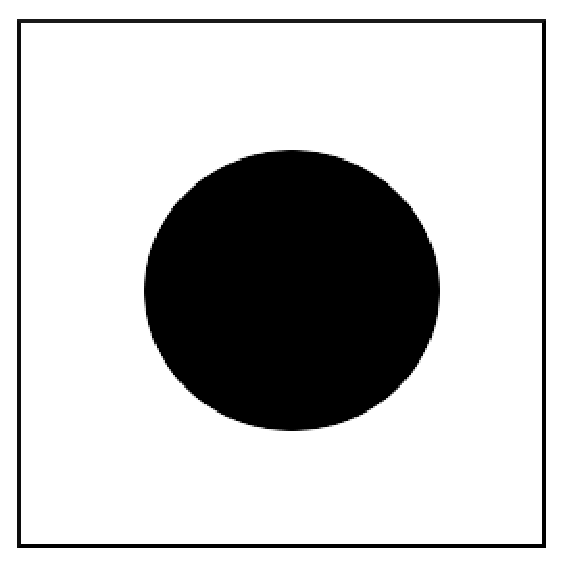
\includegraphics[scale=0.3]{images/circulo_250x250.eps}
\caption{Imagen artificial con bordes curvos entre clusters}
\label{fig:circulo}
\end{figure}

Las primeras pruebas para esta imagen consideran centroides iniciales aleatorios, y se trabajó nuevamente utilizando sólo las intensidades de gris primero y posteriormente incorporando las coordenadas de cada punto.

Los resultados obtenidos sin información espacial demuestran que el algoritmo es capaz de agrupar los puntos de manera correcta en zonas cerradas cuando existe un fuerte contraste de intensidades entre la zona interior y la exterior (figura \ref{fig:circulo_aleatorio} a y b). Al incluir las coordenadas espaciales los resultados obtenidos son diferentes. Si bien se logra diferenciar con claridad la zona central del fondo en la imagen original, se observa que las probabilidades de los puntos pertenecientes al cluster cerrado son afectadas por la distancia al centroide, que por lo que se puede observar, considerando que los puntos con valores de probabilidad más altos son los mas cercanos a éste, tiende a ubicarse en un punto tangente a la circunferencia (figura \ref{fig:circulo_aleatorio} c y d)

\begin{figure}[h]
\centering
\includegraphics[scale=0.08]{images/circulo-001.jpg}
\caption{Mapas de pertenencia con centroides iniciales aleatorios. (a - b)  sin información espacial (c - d) con información espacial.}
\label{fig:circulo_aleatorio}
\end{figure}

En la primera representación con información espacial (figura \ref{fig:circulo_aleatorio} - c) se puede ver que el rango de probabilidades para la zona circular varía desde $0,5$ tendiendo a $1$, pero sin lograr probabilidades altas, y en la segunda imagen (figura \ref{fig:circulo_aleatorio}-d) abarca probabilidades menores a $0.5$, pero no hay probabilidades nulas. A partir de la variación de colores que representan el mapa probabilístico, se observa claramente que hay incertidumbre para identificar los puntos pertenecientes a la región cerrada, y que esta incertidumbre aumenta en el resto de la imagen. Se puede apreciar además cómo las probabilidades en el fondo prácticamente recorren el rango completo, lo cual indica que la zona de fondo tampoco  es identificada con certeza como perteneciente a ningún cluster.

Luego se consideró la elección manual de los centroides iniciales: para uno de los clusters se ubicó en la zona central del círculo, mientras que para el otro fue seleccionado en el punto superior izquierdo de la imagen. No se evidencian diferencias en los resultados, y al igual que en el caso aleatorio, cuando se incluye información espacial los valores límites de probabilidades se desplazan hacia un punto tangente del objeto cerrado (figura \ref{fig:circulo_aleatorio_centr_manual}).

\begin{figure}[h]
\centering
\includegraphics[scale=0.08]{images/circulo-001.jpg}
\caption{Matriz de pertenencia, con centroide seleccionado manualmente. (a-b) sin información espacial. (c-d) con información espacial}
\label{fig:circulo_aleatorio_centr_manual}
\end{figure}

Al advertir que el resultado final era el mismo que con los centroides aleatorios,  se realizó el experimento de ejecutar el algoritmo con los centroides elegidos a mano pero con un límite de iteraciones acotado para observar cómo se desplazaban los mismos conforme las iteraciones avanzan. Como se aprecia en la figura \ref{fig:circulo_iteraciones}, inicialmente la circunferencia tiene valores cercanos a $0\%$ de pertenencia (figura \ref{fig:circulo_iteraciones}-a), pero los mismos aumentan a medida que se ejecutan más iteraciones, hasta llegar al resultado final (figura \ref{fig:circulo_iteraciones}-e), que coincide con el presentado en la figura \ref{fig:circulo_aleatorio_centr_manual}. A medida que el algoritmo progresa, el centroide se desplaza hacia un punto del borde de la circunferencia. También se puede ver que la región del fondo no logra ser identificada por el algoritmo, ya que las probabilidades abarcan el rango completo de 0 a 1. 

\begin{figure}[h]
\centering
\includegraphics[scale=0.08]{images/circulo_iteraciones_x1.jpg}
\caption{Matriz de pertenencia al primer cluster, con información espacial y selección manual de centroides iniciales. (a)Luego de 1 iteración, (b) luego de 10 iteraciones, ( c) luego de 25 iteraciones, (d) luego de 50 iteraciones, (e) luego de 100 iteraciones}
\label{fig:circulo_iteraciones}
\end{figure}

\subsection{Imágenes con ruido}
La siguiente serie de experimentos considera imágenes con ruido sal y pimienta. En la primera evaluación se utilizó una imagen con 1\% de ruido y luego se elevó al 30\% (figura \ref{fig:mitad_mitad_ruido_1p}).

\begin{figure}[H]
\centering
\includegraphics[scale=0.06]{images/original_mitad_con_ruido_1y30.jpg}
\caption{Ruido sal y pimienta 1\%}
\label{fig:mitad_mitad_ruido_1p}
\end{figure}

En caso de no incluir las coordenadas espaciales, los puntos de ruido son clasificados con una probabilidad baja de pertenencia a su clúster, debido a la diferencia de intensidad (figura \ref{fig:ruido_1y30}-a). El efecto se profundiza cuando analizamos una imagen con mayor presencia de ruido (figura \ref{fig:ruido_1y30}-b).


\begin{figure}[h]
\centering
\includegraphics[scale=0.055]{images/mitad_mitad__ruido_1y_30.jpg}
\caption{Matriz de pertenencias del cluster 1, sin información espacial. (a) con 1\% de ruido, (b) con 30\% de ruido
}
\label{fig:ruido_1y30}
\end{figure}

Contrariamente, cuando se añaden las coordenadas espaciales como otra característica al algoritmo, se obtiene una distribución general de probabilidades similar a la lograda para la imagen sin ruido (Figura \ref{fig:mitad_mitad_ruido_zoom} b-1), y al igual que en el experimento sin información espacial, los puntos con ruido son clasificados con menor probabilidad. 
En este caso, si comparamos en detalle las probabilidades obtenidas con y sin la información espacial, podemos observar que la probabilidad de pertenencia de los  puntos con ruido es más acertada cuando se utilizan las coordenadas del punto como característica adicional (Figuras \ref{fig:mitad_mitad_ruido_zoom} a-2 y b-2).


\begin{figure}[H]
\centering
\includegraphics[scale=0.05]{images/mitad_mitad_ruido_zoom-001.jpg}
\caption{Matriz de pertenencia al cluster 1, de la imagen con 1\% de ruido. 
(a-1) sin información espacial (a-2) acercamiento de región marcada en (a-1)
(b-1) con información espacial (b-2) acercamiento de región marcada en (b-1)}
\label{fig:mitad_mitad_ruido_zoom}
\end{figure}

\subsection{Imágenes con bias}
En las siguientes pruebas utilizamos una imagen con 3 regiones, correspondientes al fondo y a un objeto circular y un anillo alrededor del mismo que presentan bias (figura \ref{fig:circulo_bias}). El bias es una distorsión de la imagen causada por el instrumento de captura. Esta distorsión se presenta generalmente sobre los bordes de los objetos y causa cambios en la intensidad de los píxeles, de manera que el mismo tejido es representado por diferentes valores en la imagen \citep{juntu2005bias}.

\begin{figure}[H]
\centering
\includegraphics[scale=0.3]{images/biasing.png}
\caption{Imagen de bordes curvos con 3 clusters y bias}
\label{fig:circulo_bias}
\end{figure}

El comportamiento del algoritmo cuando no se utilizan coordenadas espaciales es similar al observado en las pruebas anteriores, las tres zonas fueron correctamente detectadas y se puede notar como el bias afecta las probabilidades de las zonas debido al cambio de intensidades  (figura \ref{fig:matriz_circulo_bias}).

\begin{figure}[H]
\centering
\includegraphics[scale=0.3]{images/bias_sin_coord.jpg}
\caption{Mapas de pertenencia sin información espacial (a) fondo (b) anillo ( c) centro}
\label{fig:matriz_circulo_bias}
\end{figure}

Cuando utilizamos coordenadas espaciales para la clasificación de esta imagen, podemos apreciar que, al igual que en los experimentos anteriores, el algoritmo no detecta correctamente la zona del fondo (figura \ref{fig:matriz_circulo_bias_espacial} a y b). En el caso particular de la imagen para el clúster del centro (figura \ref{fig:matriz_circulo_bias_espacial} - c), vemos concretamente la influencia de las coordenadas espaciales, ya que la zona central y el anillo que la rodea son reconocidos prácticamente como un solo grupo, pese a la diferencia de intensidades.

\begin{figure}[H]
\centering
\includegraphics[scale=0.3]{images/bias_con_coord.jpg}
\caption{Mapas de pertenencia con información espacial (a) cluster del fondo, zona izquierda (b) cluster del fondo, zona derecha  (c) centro}
\label{fig:matriz_circulo_bias_espacial}
\end{figure}

\subsection{Imágenes con bias y ruido}

En nuestra última prueba utilizamos una imagen con bias y ruido. En esta situación, la clusterización resultante es de menor calidad que en los experimentos anteriores debido a la presencia de una alto porcentaje de ruido así como un biasing pronunciado. 

\begin{figure}[H]
\centering
\includegraphics[scale=0.3]{images/biasing_con_ruido.png}
\caption{Imagen con bias y ruido}
\label{fig:circulo_bias_ruido}
\end{figure}

En los mapas de pertenencia de la figura \ref{fig:circulo_bias_ruido_cluster} se puede apreciar que, pese al ruido y al bias, el fondo de la imagen es correctamente clasificado (figura \ref{fig:circulo_bias_ruido_cluster}-a), pero en el segundo y tercer mapa el anillo y la parte central de la imagen original no son claramente distinguidos (figura \ref{fig:circulo_bias_ruido_cluster} b y c). Las pertenencia de la zona central y el anillo varían entre 0 y 1 y además se mezclan en determinadas zonas.

\begin{figure}[H]
\centering
\includegraphics[scale=0.3]{images/bias_sin_coord_con_ruido.jpg}
\caption{Mapa de pertenencia sin información espacial (a) cluster del  fondo (b) centro 1 (c) centro 2}
\label{fig:circulo_bias_ruido_cluster}
\end{figure}

\subsection{Análisis de costo y convergencia}
En todos los casos analizados, la curva de convergencia de la función costo tiene la forma mostrada en la Figura 17. Siempre hay un periodo inicial con un valor alto de la función costo y luego un punto de inflexión a partir del cual desciende abruptamente y los valores oscilan levemente hasta que el algoritmo se detiene, como se mencionó en la sección \ref{Introduccion}.

\begin{figure}[h]
\centering
\includegraphics[scale=0.3]{images/FALTA.png}
\caption{Curva de convergencia}
\label{fig:convergencia}
\end{figure}

